% Created 2018-05-30 Wed 05:38
% Intended LaTeX compiler: pdflatex
\documentclass[10pt]{beamer}
\usepackage[utf8]{inputenc}
\usepackage[T1]{fontenc}
\usepackage{graphicx}
\usepackage{grffile}
\usepackage{longtable}
\usepackage{wrapfig}
\usepackage{rotating}
\usepackage[normalem]{ulem}
\usepackage{amsmath}
\usepackage{textcomp}
\usepackage{amssymb}
\usepackage{capt-of}
\usepackage{hyperref}
\usetheme{Boadilla}
\author{ECON 420: Game Theory}
\date{Spring 2018}
\title{Repeated Games}
\usecolortheme{seagull}
\usefonttheme[onlylarge]{structurebold}
\usefonttheme[onlymath]{serif}
\setbeamerfont*{frametitle}{size=\normalsize,series=\bfseries}
\setbeamertemplate{navigation symbols}{}
\setbeamertemplate{itemize item}[triangle]
\setbeamertemplate{footline}{}
\setbeamertemplate{enumerate items}[default]
\hypersetup{
 pdfauthor={ECON 420: Game Theory},
 pdftitle={Repeated Games},
 pdfkeywords={},
 pdfsubject={},
 pdfcreator={Emacs 25.2.2 (Org mode 9.1.6)}, 
 pdflang={English}}
\begin{document}

\maketitle

\begin{frame}[label={sec:org2a3ee08}]{}
\alert{Announcements}
\begin{itemize}
\item Homework 4 due next Wednesday (will be posted later today)
\item Final exam: Friday, June 15 at 7:30am (!)
\end{itemize}
\end{frame}

\begin{frame}[label={sec:org85b3298}]{Prisoners' Dilemma}
\begin{center}
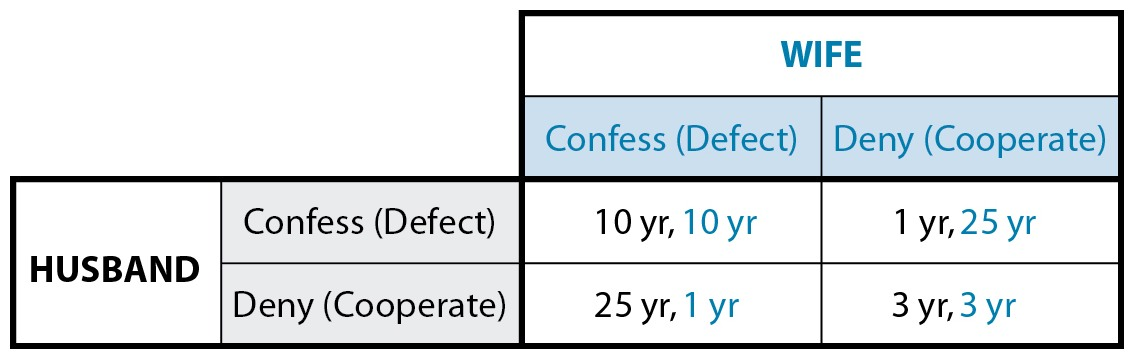
\includegraphics[width=.75\textwidth]{./img/GAMES4_FIG10.01.jpg}
\end{center}
\end{frame}

\begin{frame}[label={sec:org537aded}]{}
\alert{Game 1}
\begin{itemize}
\item You will play the prisoners' dilemma against a random opponent
\item Write your name at the top of a sheet of paper
\item Choose a strategy to play (Confess or Deny)
\item Your opponent will be randomly selected from among your classmates
\item The person(s) with the highest payoffs will receive 5 extra-credit points on the homework
\end{itemize}
\end{frame}

\begin{frame}[label={sec:org4a52643}]{Restaurant Pricing Game}
\begin{center}
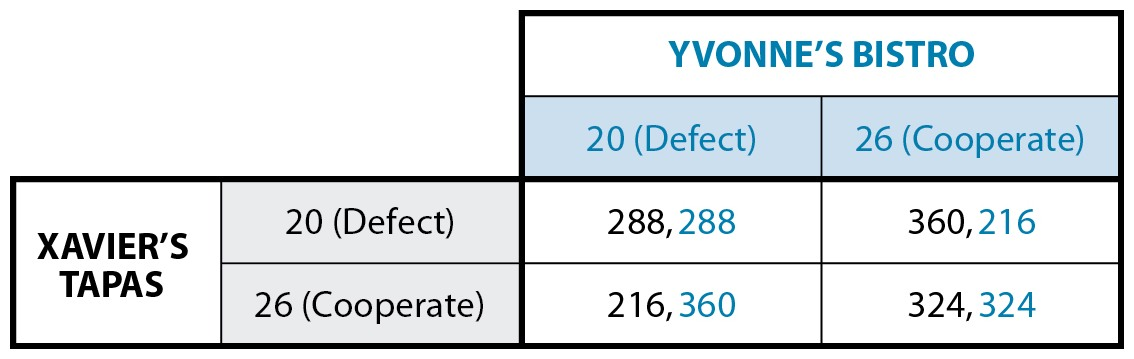
\includegraphics[width=.75\textwidth]{./img/GAMES4_FIG10.02.jpg}
\end{center}
\end{frame}

\begin{frame}[label={sec:org6648943}]{}
\alert{Game 2}
\begin{itemize}
\item Pair up with one of your classmates
\item Play the restaurant pricing game for 5 rounds
\begin{itemize}
\item Keep track of your payoffs for each round
\end{itemize}
\end{itemize}
\end{frame}

\begin{frame}[label={sec:org8f3e027}]{}
\alert{Game 3}
\begin{itemize}
\item Play the restaurant pricing game again
\begin{itemize}
\item Keep track of your payoffs each round
\end{itemize}
\item Continue playing until I say stop
\end{itemize}
\end{frame}

\begin{frame}[label={sec:orgbed9a7b}]{}
\alert{Repetition and cooperation}
\begin{itemize}
\item Which version of the game are we most likely to observe cooperation? Why?
\item Which version of the game are we \emph{least} likely to observe cooperation?
\end{itemize}
\end{frame}

\begin{frame}[label={sec:orgade0f03}]{The game tree}
\end{frame}

\begin{frame}[label={sec:orgee8a9f9}]{}
\alert{Strategies in repeated games}
\begin{itemize}
\item Strategies can be extremely complicated in repeated games 
\begin{itemize}
\item Strategies can contain infinitely many moves if the game is repeated forever!
\end{itemize}
\item Often useful to simplify the strategy to a "rule"
\item \emph{Contingent strategies}: Choose action based on action of opponent in previous round
\end{itemize}
\end{frame}

\begin{frame}[label={sec:orgf21b2b9}]{}
\alert{Rollback equilibrium}
\begin{itemize}
\item Suppose the game is played a finite number of times
\begin{itemize}
\item What is the rollback equilibrium?
\end{itemize}
\item Suppose the game is played an infinite number of times
\begin{itemize}
\item What is the rollback equilibrium?
\end{itemize}
\end{itemize}
\end{frame}

\begin{frame}[label={sec:orgbf58669}]{}
\alert{Tit-for-tat}
\begin{itemize}
\item Strategy: Cooperate in first round, then do whatever opponent does in previous round
\item Allows for cooperative outcomes, but "punishes" opponent for defecting
\end{itemize}
\end{frame}

\begin{frame}[label={sec:org68e5daa}]{}
\alert{Grim-trigger}
\begin{itemize}
\item Strategy: Cooperate in every round if opponent also cooperates, defect forever if opponent defects once
\item Most severe punishment for opponent
\end{itemize}
\end{frame}

\begin{frame}[label={sec:org2900518}]{}
\alert{Time value}
\begin{itemize}
\item Suppose the restaurant pricing game is repeated monthly
\begin{itemize}
\item Your opponent is playing a tit-for-tat strategy
\end{itemize}
\item Should you defect in the first round?
\begin{itemize}
\item Cooperate every round after
\end{itemize}
\item Gain in the first month
\item Lose \emph{more} in the second month
\item But money is more valuable today than next month!
\end{itemize}
\end{frame}

\begin{frame}[label={sec:org1ee58e9}]{}
\alert{Present value}
\begin{itemize}
\item To compare money now with money later, we need to calculate the \emph{present value} of money later
\item The PV of future money is the amount we'd be willing to accept today instead
\item For a discount rate \emph{r}, the present value of future income \emph{I} is
\end{itemize}

$$PV = \dfrac{I}{1+r}$$
\end{frame}

\begin{frame}[label={sec:org0492365}]{Example}
\end{frame}

\begin{frame}[label={sec:org5df0f40}]{}
\alert{Defecting against a grim trigger}
\begin{itemize}
\item Receive the higher payoff at first, non-cooperative outcome forever after
\item Is immediate payoff the long-run loss?
\begin{itemize}
\item What is the immediate gain?
\item What is the PV of future losses?
\end{itemize}
\end{itemize}
\end{frame}


\begin{frame}[label={sec:orgcf27c4b}]{}
\alert{Penalties and rewards}
\begin{itemize}
\item Perhaps there is a social cost to defecting (snitches get stitches?)
\item In this case, the payoff table is poorly specified
\item Properly specifying the payoffs may mean that the game is not a prisoners' dilemma at all
\item Perhaps threats or promises in a new first round can change the payoffs of a game (chapter 9)
\end{itemize}
\end{frame}

\begin{frame}[label={sec:orgdab8e35}]{}
\alert{Experiments with repeated games}
\begin{itemize}
\item Robert Axelrod created a computer "tournament" where teams could submit computer programs to play a repeated prisoners' dilemma
\item Teams chose a strategy for the programs, then they play other randomly selected programs
\begin{itemize}
\item Which strategy was best?
\end{itemize}
\item After first round, teams could submit \emph{new} strategies knowing what the optimum was
\begin{itemize}
\item Which strategy was the best this time?
\end{itemize}
\end{itemize}
\end{frame}

\begin{frame}[label={sec:orgccd13e5}]{}
\alert{Axelrod}:
\begin{itemize}
\item "Don't be envious. Don't be the first to defect. Reciprocate both cooperation and defection. Don't be too clever."
\end{itemize}
\end{frame}
\end{document}